% When does sequence order matter? An information-theoretic taxonomy of biological representation tasks
% and the limits of local encoding
% Build (in this folder): pdflatex order_taxonomy (x2); figures are read from ../figures
\documentclass[11pt]{article}
\usepackage{lmodern}
\usepackage[T1]{fontenc}
\usepackage{amsmath,amssymb,amsthm,mathtools}
\usepackage[margin=1.05in]{geometry}
\usepackage{booktabs,array}
\usepackage{microtype}
\usepackage{graphicx}
\graphicspath{{../figures/}}
\usepackage{xcolor}
\usepackage{tikz}
\usetikzlibrary{arrows.meta,positioning}
\usepackage[hidelinks]{hyperref}
\newcommand{\doi}[1]{\href{https://doi.org/#1}{\nolinkurl{doi:#1}}}
\emergencystretch=2em

\theoremstyle{plain}
\newtheorem{theorem}{Theorem}
\newtheorem{proposition}[theorem]{Proposition}
\newtheorem{corollary}[theorem]{Corollary}
\theoremstyle{definition}
\newtheorem{definition}[theorem]{Definition}
\theoremstyle{remark}
\newtheorem{remark}[theorem]{Remark}

\newcommand{\spec}{\operatorname{spec}}

\title{\bfseries When does sequence order matter?\\
An information-theoretic taxonomy of biological representation tasks\\ and the limits of local encoding}
\author{Zhengyi Chen\\[2pt]
\normalsize\begin{tabular}{c}
Guangxi Key Laboratory of Drug Discovery and Optimization,\\
Guangxi Engineering Research Center for Pharmaceutical Molecular Screening\\
and Druggability Evaluation, School of Pharmacy, Guilin Medical University,\\
Guilin 541199, P.~R.~China\\
\texttt{chenzhengyi@glmc.edu.cn}
\end{tabular}
\and
Ruqing Chen\\[2pt]
\normalsize GUT Geoservice Inc., Montreal, Qu\'ebec, Canada\\
\normalsize\texttt{ruqing@hotmail.com}}
\date{27 September 2026}

\begin{document}
\maketitle

\begin{abstract}
\noindent
Biological sequence models range from amino acid composition and $k$-mer counters to convolutional networks and
billion-parameter language models. When is a local representation sufficient, and when is global order
indispensable? We answer this question by synthesizing the spectral-fibre framework into an exact
information-theoretic taxonomy across the $20\,431$ reviewed human proteins. For any sequence $S$ of length $L$
over an alphabet of size $q$ and any local order $k$, the total combinatorial specification cost $L\log_2 q$
splits into three non-negative telescoping terms: the composition constraint $I_{\mathrm{comp}}(S)=L\log_2 q-B_1(S)$,
the resolved local-syntax information $I_{\mathrm{local}}^{(k)}(S)=B_1(S)-B_k(S)$, and the unresolved global-order
entropy $I_{\mathrm{global}}^{(k)}(S)=B_k(S)=\log_2|F_k(S)|$. Evaluating this decomposition across the human
proteome for $1\le k\le50$ reveals a sharp separation of functional classes. At $k=3$, $83.34\%$ of total order
entropy $B_1(S)$ is resolved on average, yet $99.64\%$ of human proteins ($20\,357$) retain non-trivial fibres.
By $k=5$, $99.75\%$ of $B_1(S)$ is resolved proteome-wide. Globular catalytic enzymes ($n=3\,449$) and
receptors, channels and transporters ($n=1\,816$) have median spectral resolution $\kappa=5$ ($95$th percentile
$\kappa=7$), with only $1.04\%$ and $0.77\%$ requiring $k>10$. By contrast, unresolved global order at $k>10$ is
concentrated in three architectures: C2H2 zinc-finger regulators ($n=747$, $49.13\%$ with $\kappa>10$),
structural tandem-repeat proteins ($n=199$, $39.70\%$ with $\kappa>10$ and $9.05\%$ with $\kappa>25$), and
hominoid segmental-duplication arrays ($n=67$, $74.63\%$ with $\kappa>10$ and $29.85\%$ with $\kappa>25$, $95$th
percentile $\kappa=257$). Combining this decomposition with our results on neural receptive fields, clinical
variant copy ambiguity, zinc-finger specificity, benchmark drift ratios and symmetry quotients yields a concrete
decision rule for choosing sequence encoders in computational biology.
\end{abstract}

\medskip
\noindent\textbf{Keywords.} sequence representation, spectral fibre, fibre entropy, spectral resolution, human
proteome, local encoders, protein language models, repeat proteins, representation selection.

% ================================================================ 1
\section{Introduction}\label{sec:intro}

A central choice in computational biology is how to represent a biomolecular sequence or graph. Historically,
two traditions have competed. The first builds fixed-length vectors from local subword or subgraph statistics:
amino acid and $k$-mer composition, amphiphilic pseudo amino acid composition (PseAAC) \cite{Chou05}, extended-connectivity
molecular fingerprints (ECFP) \cite{Morgan65,RH10}, and one-dimensional convolutional networks (CNNs) with global
pooling \cite{DeepBind,Kim14}. The second relies on architectures with global context—recurrent networks,
state-space models \cite{S4,Mamba}, and Transformers with positional encodings \cite{Vaswani17,ESM2,ProtTrans}—to
capture long-range order.

Empirically, simple local models often match deep language models on bulk classification benchmarks (such as
subcellular localization, broad enzyme family assignment or physicochemical property regression), yet fail
catastrophically on tasks that depend on the arrangement of repeated domains or the exact copy index of a
variant. Without a formal theory, this divide has remained a matter of trial and error.

In a series of companion studies \cite{CC26a,CC26b,CC26c,CC26d,CC26e,CC26f,CC26g,CC26h}, we developed an exact
combinatorial and algebraic theory of what local representations can and cannot see. Any encoder that depends on
a sequence $S$ only through its multiset of $k$-mers (and boundary $(k-1)$-mers) factors through the quotient map
$\pi_k$, and is therefore constant on the \emph{spectral fibre} $F_k(S)=\pi_k^{-1}(\pi_k(S))$. The cardinality
$N_k(S)=|F_k(S)|$ of this fibre is the number of Eulerian trails of the de~Bruijn multigraph $G_k(S)$, given in
closed form by the BEST theorem \cite{BEST,Pev95,Ukk92}.

This closing paper of the series synthesizes these results into a quantitative, proteome-wide taxonomy of
sequence order information. Our contributions are three:
\begin{enumerate}
\item \emph{Exact three-term information decomposition} (Section~\ref{sec:decomposition}): we formulate the
pointwise telescoping identity $L\log_2 q = I_{\mathrm{comp}}(S) + I_{\mathrm{local}}^{(k)}(S) + I_{\mathrm{global}}^{(k)}(S)$
and evaluate it exactly across all $20\,431$ reviewed human proteins for $15$ orders from $k=1$ to $k=50$
(Table~\ref{tab:decomp}).
\item \emph{Functional taxonomy of order regimes} (Section~\ref{sec:taxonomy}): we partition the human proteome into
six functional and structural classes and show that non-repetitive globular enzymes and membrane receptors collapse
to unique sequences by $k\approx7$--$10$, whereas transcriptional zinc-finger arrays, structural repeats and
segmental-duplication families form a heavy tail of unresolved global order (Table~\ref{tab:classes},
Figure~\ref{fig:taxonomy}).
\item \emph{Synthesis and architectural selection guide} (Sections~\ref{sec:synthesis} and~\ref{sec:guide}): we
integrate the findings of all eight studies—from convolutional invariance theorems and ClinVar copy ambiguity to
C2H2 zinc-finger reorderings, FibreBench language-model evaluations and double-stranded/molecular symmetry
quotients—into a practical design rule for biological machine learning (Table~\ref{tab:series}).
\end{enumerate}

% ================================================================ 2
\section{The three-part decomposition of sequence information}\label{sec:decomposition}

Let $\Sigma$ be a finite alphabet of size $q=|\Sigma|$ ($q=20$ for standard amino acids), and let $S\in\Sigma^L$ be
a sequence of length $L$. Specifying $S$ among all $q^L$ possible strings of length $L$ requires
\[
I_{\mathrm{total}}(S)=\log_2(q^L)=L\log_2 q\quad\text{bits}
\]
($4.3219\,L$ bits for proteins).

Recall from \cite{CC26c} that the spectral fibre $F_k(S)$ at order $k\ge1$ is the set of sequences $T\in\Sigma^L$
having the same $k$-mer multiset $\spec_k(T)=\spec_k(S)$ and the same prefix $T[1..k-1]=S[1..k-1]$. Because the
quotient maps refine one another as $k$ increases, the fibres form a nested chain of subsets:
\[
\Sigma^L \;\supset\; F_1(S) \;\supseteq\; F_2(S) \;\supseteq\; \cdots \;\supseteq\; F_{\kappa(S)}(S)=\{S\},
\]
where $F_1(S)$ is the set of all permutations of $S$ preserving its amino acid counts $\{c_a(S)\}_{a\in\Sigma}$,
of size $N_1(S)=L!\big/\prod_{a\in\Sigma}c_a(S)!$, and $\kappa(S)=\min\{k:N_k(S)=1\}$ is the \emph{spectral
resolution} of $S$ \cite{CC26a,CC26b}. Write $B_k(S)=\log_2 N_k(S)$ for the \emph{fibre entropy} at order $k$, i.e.\
the number of bits of sequence identity that remain unresolved once the $k$-spectrum of $S$ is fixed \cite{CC26c}.

\begin{theorem}[pointwise telescoping decomposition of sequence information]\label{thm:decomp}
For every sequence $S\in\Sigma^L$ and every order $1\le k\le L$, the total specification cost $I_{\mathrm{total}}(S)$
decomposes into three non-negative terms:
\begin{equation}\label{eq:decomp}
L\log_2 q \;=\; \underbrace{\bigl(L\log_2 q - B_1(S)\bigr)}_{I_{\mathrm{comp}}(S)}
\;+\; \underbrace{\bigl(B_1(S) - B_k(S)\bigr)}_{I_{\mathrm{local}}^{(k)}(S)}
\;+\; \underbrace{B_k(S)}_{I_{\mathrm{global}}^{(k)}(S)}.
\end{equation}
Moreover:
\begin{enumerate}
\item $I_{\mathrm{comp}}(S)=\log_2\bigl(q^L/N_1(S)\bigr)\ge0$ depends only on the $1$-mer composition of $S$; it is
the information captured by a bag-of-residues encoder ($k=1$).
\item $I_{\mathrm{local}}^{(k)}(S)=\log_2\bigl(N_1(S)/N_k(S)\bigr)\ge0$ is monotone non-decreasing in $k$, equals $0$
at $k=1$, and equals $B_1(S)$ for all $k\ge\kappa(S)$; it is the exact order information resolved by refining from
composition to $k$-mer statistics. Further, $I_{\mathrm{local}}^{(k)}(S)=\sum_{j=1}^{k-1}\Delta B_j(S)$, where
$\Delta B_j(S)=B_j(S)-B_{j+1}(S)\ge0$ is the incremental information gained at scale $j+1$.
\item $I_{\mathrm{global}}^{(k)}(S)=B_k(S)\ge0$ is monotone non-increasing in $k$ and vanishes if and only if
$k\ge\kappa(S)$; it is the exact conditional entropy $H(X\mid\pi_k(X)=\pi_k(S))$ for $X$ uniform on $F_k(S)$, i.e.\
the global order information to which every order-$k$ local encoder is provably blind \cite{CC26c,CC26d}.
\end{enumerate}
\end{theorem}

\begin{proof}
Algebraic identity~\eqref{eq:decomp} is immediate by cancelling $B_1(S)$ and $B_k(S)$. Non-negativity and
monotonicity follow from the chain of inclusions $\{S\}\subseteq F_k(S)\subseteq F_{k-1}(S)\subseteq F_1(S)\subseteq\Sigma^L$,
which gives $1\le N_k(S)\le N_{k-1}(S)\le N_1(S)\le q^L$ and hence $0\le B_k(S)\le B_{k-1}(S)\le B_1(S)\le L\log_2 q$.
Equality $B_k(S)=0$ holds if and only if $N_k(S)=1$, which by definition is $k\ge\kappa(S)$.
\end{proof}

\begin{table}[t]
\centering\footnotesize\setlength{\tabcolsep}{3.5pt}
\begin{tabular}{rrrrrrrr}
\toprule
order $k$ & med.\ $I_{\mathrm{comp}}/L$ & mean $I_{\mathrm{local}}^{(k)}/L$ & mean $B_k/L$
 & mean $I_{\mathrm{local}}^{(k)}/B_1$ & mean $B_k/B_1$ & proteins with & share with\\
 & (bits/res.) & (bits/res.) & (bits/res.) & (\%) & (\%) & $B_k(S)>0$ & $B_k(S)>0$\\
\midrule
1  & 0.3947 & 0.0000 & 3.8736 &   0.000\% & 100.000\% & 20\,431 & 100.00\%\\
2  & 0.3947 & 1.3278 & 2.5458 &  34.774\% &  65.226\% & 20\,422 &  99.96\%\\
3  & 0.3947 & 3.2204 & 0.6532 &  83.342\% &  16.658\% & 20\,357 &  99.64\%\\
4  & 0.3947 & 3.8016 & 0.0720 &  98.145\% &   1.855\% & 18\,391 &  90.02\%\\
5  & 0.3947 & 3.8643 & 0.0094 &  99.749\% &   0.251\% &  9\,504 &  46.52\%\\
6  & 0.3947 & 3.8701 & 0.0035 &  99.903\% &   0.097\% &  3\,445 &  16.86\%\\
8  & 0.3947 & 3.8722 & 0.0014 &  99.962\% &   0.038\% &  1\,346 &   6.59\%\\
10 & 0.3947 & 3.8729 & 0.0007 &  99.981\% &   0.019\% &    854  &   4.18\%\\
12 & 0.3947 & 3.8732 & 0.0004 &  99.989\% &   0.011\% &    614  &   3.01\%\\
16 & 0.3947 & 3.8735 & 0.0001 &  99.996\% &   0.004\% &    327  &   1.60\%\\
20 & 0.3947 & 3.8735 & 0.0001 &  99.998\% &   0.002\% &    194  &   0.95\%\\
25 & 0.3947 & 3.8736 & 0.0000 &  99.999\% &   0.001\% &    114  &   0.56\%\\
30 & 0.3947 & 3.8736 & 0.0000 &  99.999\% &   0.001\% &     81  &   0.40\%\\
40 & 0.3947 & 3.8736 & 0.0000 & 100.000\% &   0.000\% &     50  &   0.24\%\\
50 & 0.3947 & 3.8736 & 0.0000 & 100.000\% &   0.000\% &     37  &   0.18\%\\
\bottomrule
\end{tabular}
\caption{Exact decomposition of sequence information across the $20\,431$ reviewed human proteins of UniProt for
orders $1\le k\le50$. Total specification cost is $\log_2 20\approx4.3219$ bits per residue.}\label{tab:decomp}
\end{table}

Table~\ref{tab:decomp} evaluates Theorem~\ref{thm:decomp} across all $20\,431$ reviewed human proteins. Three
quantitative facts stand out:
\begin{enumerate}
\item \emph{Composition alone is a small fraction of sequence identity.} Fixing the amino acid counts ($k=1$)
accounts for a median of $0.3947$ bits per residue (about $9.1\%$ of $\log_2 20$, coming from deviations from a
uniform amino acid distribution and Stirling's correction), leaving a mean of $3.8736$ bits per residue in the
permutation entropy $B_1(S)$.
\item \emph{Short-range transitions ($k=2$ to $5$) absorb over $99.7\%$ of bulk permutation entropy.} Dipeptides
($k=2$) resolve $34.77\%$ of $B_1(S)$; tripeptides ($k=3$) resolve $83.34\%$; tetrapeptides ($k=4$) resolve
$98.14\%$; and pentapeptides ($k=5$) resolve $99.75\%$. This explains why $3$-mer to $5$-mer composition vectors
and shallow CNNs perform strongly on bulk proteome-wide benchmarks: on average, almost all permutation freedom is
eliminated by $k=5$.
\item \emph{Bulk averages hide a persistent unresolved tail.} Even though mean $B_k/B_1$ is only $16.66\%$ at $k=3$
and $0.25\%$ at $k=5$, $99.64\%$ of human proteins still have $B_3(S)>0$, $46.52\%$ ($9\,504$ proteins) have
$B_5(S)>0$, $4.18\%$ ($854$ proteins) have $B_{10}(S)>0$, and $0.56\%$ ($114$ proteins) have $B_{25}(S)>0$.
\end{enumerate}

% ================================================================ 3
\section{A proteome-wide taxonomy of order regimes}\label{sec:taxonomy}

To see which biological functions sit in which order regime, we partitioned the $20\,431$ reviewed human proteins
into six non-overlapping classes based on UniProt family and functional annotations (Table~\ref{tab:classes} and
Figure~\ref{fig:taxonomy}).

\begin{table}[t]
\centering\footnotesize\setlength{\tabcolsep}{3.5pt}
\begin{tabular}{>{\raggedright\arraybackslash}p{0.29\textwidth}rrrrrrrr}
\toprule
functional / structural class & proteins & med.\ $L$ & mean & mean & $\kappa>5$ & $\kappa>10$ & $\kappa>25$ & med. / p95\\
 & $n$ & (aa) & $B_3/B_1$ & $B_5/B_1$ & share & share & share & $\kappa(S)$\\
\midrule
Catalytic enzymes & $3\,449$ & 481 & 17.28\% & 0.09\% & 42.22\% & 1.04\% & 0.17\% & 5 / 7\\
Receptors, channels and transporters & $1\,816$ & 410 & 17.23\% & 0.08\% & 43.01\% & 0.77\% & 0.11\% & 5 / 7\\
Other globular and cellular proteins & $14\,153$ & 380 & 16.23\% & 0.19\% & 45.00\% & 2.18\% & 0.35\% & 5 / 8\\
\midrule
C2H2 zinc-finger regulators & $747$ & 560 & 17.80\% & 1.40\% & 88.49\% & 49.13\% & 2.54\% & 10 / 23\\
Structural tandem-repeat proteins & $199$ & 195 & 25.80\% & 4.14\% & 86.43\% & 39.70\% & 9.05\% & 10 / 41\\
Segmental-duplication arrays & $67$ & 638 & 19.99\% & 1.70\% & 97.01\% & 74.63\% & 29.85\% & 16 / 257\\
\bottomrule
\end{tabular}
\caption{Information decomposition and spectral resolution $\kappa(S)$ across six classes of the human proteome.
The upper three classes follow the random-sequence law $\kappa\sim2\log_{20}L+O(1)$ ($95$th percentile $\kappa\le8$);
the lower three classes form the repeat-driven tail.}\label{tab:classes}
\end{table}

\begin{figure}[t]
\centering
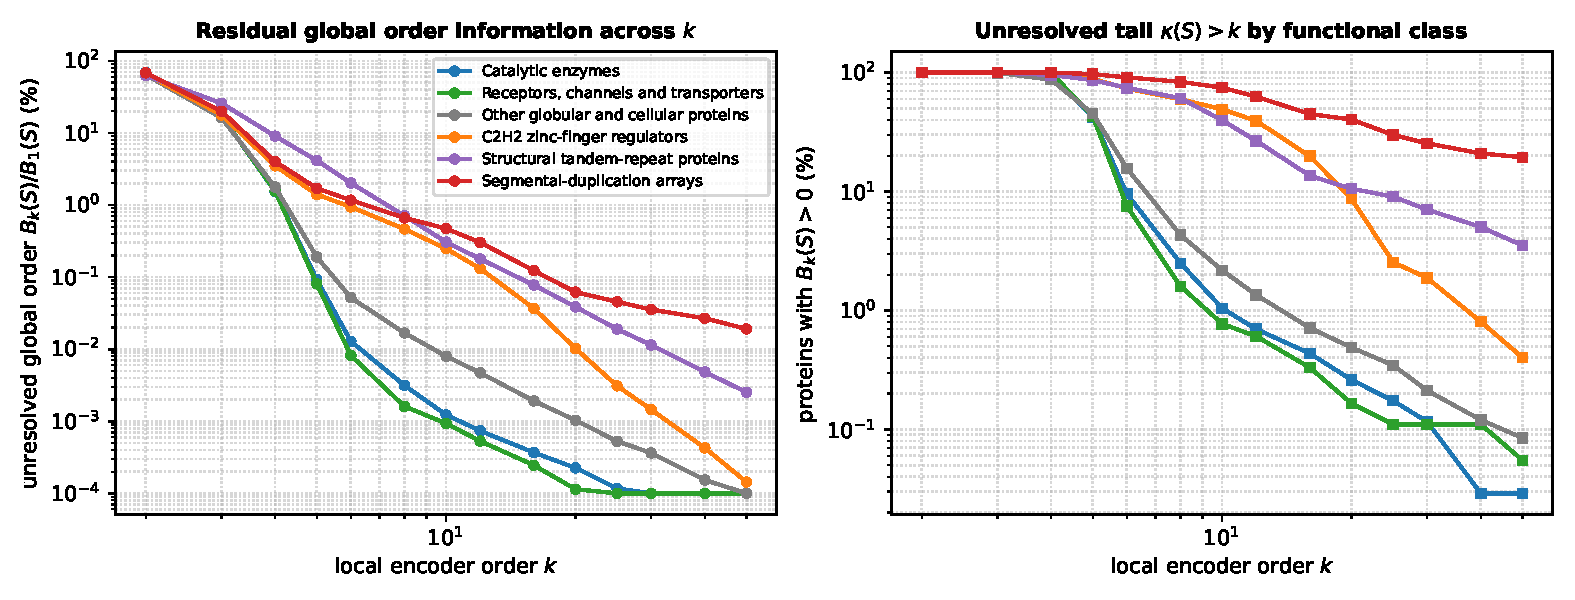
\includegraphics[width=\textwidth]{fig_taxonomy.pdf}
\caption{Left: mean unresolved global order $B_k(S)/B_1(S)$ (\%) as a function of local encoder order $k$ across
the six protein classes. Right: percentage of proteins in each class whose sequence remains unresolved at order $k$
($B_k(S)>0$, i.e.\ $\kappa(S)>k$).}\label{fig:taxonomy}
\end{figure}

Table~\ref{tab:classes} and Figure~\ref{fig:taxonomy} establish three natural regimes of sequence encoding:

\paragraph{Regime I: Composition-dominated and short-motif tasks ($k=1$ to $5$).}
Bulk physicochemical properties (molecular weight, isoelectric point, average hydropathy, overall charge) are
exact functions of the $1$-mer spectrum ($k=1$). Short linear targeting motifs and cleavage sites reside at $k=3$
to $5$. At $k=3$, however, every class still retains $16$--$26\%$ of its order entropy $B_1(S)$, and a single
protein of $300$ residues can have $2^{239}$ Eulerian reconstructions \cite{CC26b}. Thus $k=3$ separates reference
proteins empirically while leaving individual sequences heavily under-determined.

\paragraph{Regime II: Globular enzymes and membrane receptors ($k=5$ to $10$).}
For catalytic enzymes ($n=3\,449$), membrane receptors, ion channels and transporters ($n=1\,816$), and general
globular proteins ($n=14\,153$), the residual order entropy $B_5/B_1$ drops below $0.2\%$ at $k=5$. Their median
spectral resolution is $\kappa=5$, and $95\%$ of all enzymes and receptors are uniquely reconstructed from their
$7$-mer spectrum ($\text{p95 }\kappa=7$; over $98.9\%$ by $k=10$). Because globular folds avoid long exact repeats to
prevent misfolding and aggregation, their sequences obey the random-sequence scaling $\kappa(S)\approx2\log_{20}L$.
For phenotypes on these classes, a local receptive field of $R\ge10$ is injective on over $98.9\%$ of wild-type
proteins.

\paragraph{Regime III: Repeat-array and long-range order tasks ($k>10$ to $k>25$).}
The three lower classes in Table~\ref{tab:classes} violate random-sequence scaling by up to two orders of magnitude:
\begin{itemize}
\item \emph{C2H2 zinc-finger regulators ($n=747$, including KRAB-ZFPs):} $88.49\%$ require $k>5$, $49.13\%$ require
$k>10$, and $2.54\%$ ($19$ proteins in this broader class; $17$ with annotated canonical C2H2 domains in \cite{CC26f})
require $k>25$. Their median $\kappa$ is $10$ and their $95$th percentile is $23$, driven by conserved linker-helix
repeats and recent tandem finger duplications.
\item \emph{Structural tandem-repeat proteins ($n=199$, mucins, collagens, keratin-associated proteins, filaggrin):}
mean $B_3/B_1$ is $25.80\%$, $39.70\%$ require $k>10$, $9.05\%$ require $k>25$, and $\text{p95 }\kappa=41$.
\item \emph{Hominoid segmental-duplication arrays ($n=67$, NBPF, GOLGA6, NPIP, POTE):} $74.63\%$ require $k>10$,
$29.85\%$ require $k>25$, median $\kappa=16$, and $\text{p95 }\kappa=257$ (reaching $\kappa=560$ in NBPF20
\cite{CC26b}).
\end{itemize}

% ================================================================ 4
\section{Synthesis across the eight-part series}\label{sec:synthesis}

Table~\ref{tab:series} summarizes how the seven companion studies and the present work fit together as a single
mathematical and empirical programme.

\begin{table}[t]
\centering\footnotesize\setlength{\tabcolsep}{4pt}
\renewcommand{\arraystretch}{1.15}
\begin{tabular}{>{\raggedright\arraybackslash}p{0.05\textwidth}>{\raggedright\arraybackslash}p{0.23\textwidth}>{\raggedright\arraybackslash}p{0.31\textwidth}>{\raggedright\arraybackslash}p{0.34\textwidth}}
\toprule
part & focus & core mathematical object & principal empirical finding\\
\midrule
I \cite{CC26a,CC26b} & Proteome spectral atlas \& Separation $\ne$ Resolution & De~Bruijn multigraph $G_k(S)$, BEST count $N_k(S)$, resolution $\kappa(S)$ & $100\%$ of unique human proteins separated at $k=3$, yet $99.64\%$ unresolved ($854$ at $k=10$, $114$ at $k=25$)\\
II \cite{CC26c} & Quotient geometry \& information loss & Quotient lattice $(\mathcal L,\preceq)$, fibre entropy $B_k(S)$, diameter $D_k(S)$ & Exact mutual-information ceiling $H(S)-\mathbb E[B_k]$ and Fano error lower bound; $D_k(S)=\Theta(L)$\\
III \cite{CC26d} & Neural architectural boundaries & Window integral $\int F\,d\mu_S^R$; symmetric vs.\ sign-aware relative bias; SSM tail bound & $15$ PyTorch architectures tested in float64 ($2\,700$ pairs): zero violations; attention pooling \& symmetric clip stay in $F_R$\\
IV \cite{CC26e} & Genomic reachability \& ClinVar variants & Transition operators $\mathcal M_{\mathrm{genomic}}$, reachable fibre $F_k^{\mathrm{bio}}$, copy twins & Single variants leave $F_k$; $36.5\%$ copy ambiguity in NBPF at $k=10$; strong depletion in ClinVar ($4$ P/LP twins at $k=10$, $0$ at $k=25$)\\
V \cite{CC26f} & Phenotypic insufficiency (C2H2 zinc fingers) & Finger-multiset conservation ($k\ge24$), block swap across $(k-1)$-mers & $883/1\,178$ ($75\%$) $k=25$ mates across $17$ C2H2 proteins reorder recognition helices ($17/31$ in ZNF91); KLF18 negative control\\
VI \cite{CC26g} & FibreBench evaluation of protein language models & Same-protein substitution yardstick, drift ratio $\rho=\Delta_{\mathrm{fibre}}/\Delta_{\mathrm{sub}}$ & Across $258$ pairs ($1\,016$ sequences), ESM-2 ($8$M--$650$M) median $\rho=0.49$--$0.81$ at $k=25$ ($70\%$ sub-mutational)\\
VII \cite{CC26h} & Symmetry-constrained fibres (DNA \& ECFP) & $\mathbb Z/2$ $(-1)$-eigenlattice $\Lambda^-$ on double cover; coarsened symmetric window $\Omega_r$ & $\phi$X174 $|\mathrm{DS}(S,10)|=3.19\cdot10^{13}$ vs.\ $1.37\cdot10^{36}$ double-cover circuits; exact RDKit ECFP4/6 collision pairs\\
VIII & Information decomposition \& selection guide & Telescoping identity $L\log_2 q = I_{\mathrm{comp}}+I_{\mathrm{local}}^{(k)}+B_k$ & Globular enzymes/receptors resolve by $\kappa\le7$ ($\text{p95}$); repeat families form the $k>10$ tail; four-step practitioner guide\\
\bottomrule
\end{tabular}
\caption{Overview of the eight-paper programme on the spectral fibres of biological sequence and molecular
encoders.}\label{tab:series}
\end{table}

Together, the eight studies establish four cross-cutting principles:
\begin{enumerate}
\item \emph{Empirical separation on a dataset does not imply injectivity on sequence space} (Parts~I--II). A
representation can assign distinct vectors to all $20\,375$ distinct human reference sequences at $k=3$ while
collapsing $2^{100}$ or more alternative Eulerian arrangements onto each sequence's vector.
\item \emph{Architectural complexity does not break locality without asymmetric positional input} (Part~III).
Adding depth, residual connections, gating, attention pooling, unpositioned self-attention or symmetrically clipped
relative biases only changes the effective window $R$; escaping $F_R$ requires absolute positions, strides,
sign-aware/unclipped relative biases, or non-decaying state spaces.
\item \emph{Even escaping architectures suffer from pooling attenuation on long repeats} (Part~VI). Although ESM-2
(RoPE) and ProtBERT (absolute position) lie outside the invariant class in principle, global mean pooling averages
out phase shifts across transposed blocks, leaving $70\%$ of $k=25$ fibre rearrangements smaller in embedding shift
than a single amino acid substitution.
\item \emph{Where local models are blind, short-read clinical databases are also nearly blind} (Parts~IV--V).
Order-$25$ fibre rearrangements dramatically alter predicted DNA-binding motifs in KRAB zinc-finger proteins
(Part~V), and copy-ambiguous twin positions cover $23$--$37\%$ of mucins and NBPF proteins (Part~IV). Yet in
ClinVar, copy-ambiguous pathogenic missense variants are depleted to $4$ at $k=10$ and $0$ at $k=25$, because
short-read sequencing discards multi-mapping reads in identical repeats.
\end{enumerate}

% ================================================================ 5
\section{A practitioner's decision rule for sequence representation}\label{sec:guide}

For a given biological prediction problem with target phenotype $Y\colon\mathcal X\to\mathcal Y$ on a protein or
nucleic-acid class $\mathcal X$, our results reduce encoder selection to four verifiable checks:

\begin{enumerate}
\item \textbf{Check the spectral resolution $\kappa(\mathcal X)$ of the target sequences.}
Compute $\kappa(S)$ (in $O(L\log L)$ time via suffix arrays or de~Bruijn Eulerian degree checks) for the sequences
in $\mathcal X$. If the target class consists of globular enzymes, transporters or non-repetitive cellular proteins,
$95\%$ of sequences satisfy $\kappa(S)\le7$ and $99\%$ satisfy $\kappa(S)\le10$ (Table~\ref{tab:classes}). Any
encoder with receptive field $R\ge10$ is injective on almost the entire domain.
\item \textbf{Check phenotypic sufficiency on the fibre $F_R(S)$.}
If $\mathcal X$ contains repeat proteins with $\kappa(S)>R$, test whether the target phenotype $Y$ is invariant
under elementary fibre moves (exchanging segments bounded by repeated $(R-1)$-mers, or swapping homologous variants
between identical repeat copies). For bulk stability or composition-driven properties, $Y$ is approximately
fibre-invariant and local encoders suffice. For order-sensitive phenotypes—such as tandem C2H2 zinc-finger DNA
specificity (Part~V) or domain-specific pathogenic mutations in repeat arrays (Part~IV)—any encoder confined to
$F_R$ incurs an irreducible error of at least $\frac12\,d(Y(S),Y(T))$ (Part~V, Theorem~4).
\item \textbf{Choose an escaping mechanism that matches the read-out.}
When $R<\kappa(S)$ and $Y$ is order-sensitive, do not rely on deeper stride-1 convolutions, attention pooling or
symmetrically clipped relative biases (Part~III, Table~1). Include absolute positional encodings, sign-aware
or unclipped relative encodings (Shaw, T5, RoPE, ALiBi), or long-memory state-space layers ($\rho\to1$).
\item \textbf{Avoid global mean pooling when domain order or copy index is the signal.}
As FibreBench demonstrates (Part~VI), even a $650$M-parameter RoPE Transformer loses most of its sensitivity to
block transpositions when its residue states are collapsed by global mean pooling ($\text{median }\rho=0.81<1$).
Use position-retaining read-outs (per-residue heads, cross-attention to positional queries, or flattened/strided
read-outs) whenever the downstream task depends on which repeat copy is modified or how repeat domains are ordered.
\end{enumerate}

\section*{Data and code availability}
The script \texttt{code/order\_taxonomy.py} computes the exact information decomposition (Table~\ref{tab:decomp}),
the functional class breakdown (Table~\ref{tab:classes}) and Figure~\ref{fig:taxonomy} from the proteome fibre
catalogue, writing \texttt{results/order\_taxonomy\_output.txt} and
\texttt{results/order\_taxonomy\_summary.json}. Code, results and manuscript sources are available at
\url{https://github.com/Ruqing1963/order-taxonomy}.

\section*{Funding}
This project was supported by the National Natural Science Foundation of China (No.~22464010), the
Guangxi Natural Science Foundation of China (No.~2025GXNSFAA069294), and the 2025 Bagui Youth Top
Talent Project.

\small
\begin{thebibliography}{99}
\bibitem{BEST} T.~van Aardenne-Ehrenfest, N.~G.~de Bruijn, \emph{Circuits and trees in oriented linear
graphs}, Simon Stevin \textbf{28} (1951) 203--217.
\bibitem{DeepBind} B.~Alipanahi, A.~Delong, M.~T.~Weirauch, B.~J.~Frey, \emph{Predicting the sequence
specificities of DNA- and RNA-binding proteins by deep learning}, Nat.\ Biotechnol.\ \textbf{33} (2015)
831--838. \doi{10.1038/nbt.3300}
\bibitem{CC26a} Z.~Chen, R.~Chen, \emph{What a local encoder cannot see: spectral fibres of the human proteome
and the representation of perturbagens}, Zenodo (2026). \doi{10.5281/zenodo.22950095}
\bibitem{CC26b} Z.~Chen, R.~Chen, \emph{Separation without resolution: the spectral fibre geometry of the human
proteome and the blind spots of local sequence encoders}, Zenodo (2026). \doi{10.5281/zenodo.22959211}
\bibitem{CC26c} Z.~Chen, R.~Chen, \emph{Information loss and quotient geometry of local sequence encoders:
representation lattices, fibre entropy and diameter bounds}, Zenodo (2026). \doi{10.5281/zenodo.22960439}
\bibitem{CC26d} Z.~Chen, R.~Chen, \emph{What finite-receptive-field encoders cannot distinguish: invariance
theorems and architectural boundaries of convolutional sequence models}, Zenodo (2026).
\doi{10.5281/zenodo.22963882}
\bibitem{CC26e} Z.~Chen, R.~Chen, \emph{Biologically reachable spectral fibres: repeat shuffling, copy
ambiguity and the scarcity of cryptic pathogenic missense variants in ClinVar}, Zenodo (2026).
\doi{10.5281/zenodo.22966020}
\bibitem{CC26f} Z.~Chen, R.~Chen, \emph{Phenotypic insufficiency of local protein representations:
fibre-preserving rearrangements of human C2H2 zinc-finger arrays reorder DNA-recognition residues under an
invariant 25-spectrum}, Zenodo (2026). \doi{10.5281/zenodo.22967128}
\bibitem{CC26g} Z.~Chen, R.~Chen, \emph{FibreBench: stress-testing protein sequence encoders against exact
combinatorial spectral invariants}, Zenodo (2026). \doi{10.5281/zenodo.22968831}
\bibitem{CC26h} Z.~Chen, R.~Chen, \emph{Symmetry-constrained spectral fibres: reverse-complement group actions
on double-stranded DNA and the fibres of circular molecular fingerprints}, Zenodo (2026).
\bibitem{Chou05} K.-C.~Chou, \emph{Using amphiphilic pseudo amino acid composition to predict enzyme subfamily
classes}, Bioinformatics \textbf{21} (2005) 10--19. \doi{10.1093/bioinformatics/bth466}
\bibitem{ProtTrans} A.~Elnaggar et al., \emph{ProtTrans: toward understanding the language of life through
self-supervised learning}, IEEE Trans.\ Pattern Anal.\ Mach.\ Intell.\ \textbf{44} (2022) 7112--7127.
\doi{10.1109/TPAMI.2021.3095381}
\bibitem{Mamba} A.~Gu, T.~Dao, \emph{Mamba: linear-time sequence modeling with selective state spaces},
arXiv:2312.00752 (2023).
\bibitem{S4} A.~Gu, K.~Goel, C.~R\'e, \emph{Efficiently modeling long sequences with structured state spaces},
International Conference on Learning Representations (2022).
\bibitem{Kim14} Y.~Kim, \emph{Convolutional neural networks for sentence classification}, Proc.\ EMNLP (2014)
1746--1751. \doi{10.3115/v1/D14-1181}
\bibitem{ESM2} Z.~Lin et al., \emph{Evolutionary-scale prediction of atomic-level protein structure with a
language model}, Science \textbf{379} (2023) 1123--1130. \doi{10.1126/science.ade2574}
\bibitem{Morgan65} H.~L.~Morgan, \emph{The generation of a unique machine description for chemical
structures: a technique developed at Chemical Abstracts Service}, J.\ Chem.\ Doc.\ \textbf{5} (1965) 107--113.
\doi{10.1021/c160017a018}
\bibitem{Pev95} P.~A.~Pevzner, \emph{DNA physical mapping and alternating Eulerian cycles in colored
graphs}, Algorithmica \textbf{13} (1995) 77--105. \doi{10.1007/bf01188582}
\bibitem{RH10} D.~Rogers, M.~Hahn, \emph{Extended-connectivity fingerprints}, J.\ Chem.\ Inf.\ Model.\
\textbf{50} (2010) 742--754. \doi{10.1021/ci100050t}
\bibitem{Ukk92} E.~Ukkonen, \emph{Approximate string-matching with $q$-grams and maximal matches},
Theoret.\ Comput.\ Sci.\ \textbf{92} (1992) 191--211. \doi{10.1016/0304-3975(92)90143-4}
\bibitem{Vaswani17} A.~Vaswani et al., \emph{Attention is all you need}, Advances in Neural Information
Processing Systems (2017).
\end{thebibliography}

\end{document}